\chapter{Predictive Analytics im öffentlichen Sektor}

% TODO
% Stand Entscheidungshilfen (wie vorstellbar: Mensch entscheidet, Computer
%   unterstützt)
% Abgrenzung zum privaten Sektor
% auf operativer Ebene allerdings ähnlich

% s. Watson, Abschnitt Lack of regulation and algorithm bias
% TODO bias insgesamt (in Rahmenbedingungen)
\begin{figure}%[!hbt]
\centering
\caption{Risikomatrix für die Nutzung maschineller Entscheidungshilfen}
\includegraphics[scale=1.0]{Grafiken/Risk_Matrix_Ink.pdf} 
\label{pic:Risiko_Matrix}
\end{figure}

\section{Rahmenbedingungen}

% TODO
% Rahmenbedingungen:
% - Wahrheit taktisch genutzt
% - versch. Gruppen/Kulturen -> versch. Wahrheiten
% - Themen kontroverser (vs. z. B. Fruchtsäfte)
% - Konkurrenz (v. a. bei strategischen Entscheidungen) 
% - Ignorieren (-> Probleme menschl. Urteile)

%-------------------------------------------------------------------------------
Tetlock ist der Meinung, dass die Kernaufgabe politischer Weltanschauungen
nicht die Erstellung möglichst korrekter Prognosen ist, sondern die
Aufrechterhaltung einer bequemen Illusion von Berechenbarkeit
(vgl. \cite{Tetlock}, S.~39). Somit sind die Ergebnisse schlecht, weil keine
genaue Abbildung der Realität beabsichtigt wird. Die Aufrechterhaltung von
Glaubenssätzen, die zum kollektiven Zusammenhalt beitragen, hat höhere
Priorität.

In diesem Zusammenhang sind auch verschiedene Interpretationen des
Wahrheitsbegriffs bedeutsam. Eine weit verbreitete Interpretation wird mit
Hilfe des Pragmatismus von William James definiert. Demnach werden
Aussagen von Menschen als Wahrheit akzeptiert, falls die Aussagen ihnen bei der
Orientierung in der Welt nützlich sind. Dies liefert eine Erklärung dafür, dass
Menschen dazu tendieren Aussagen zu glauben, die ihre eigene Weltsicht
bestätigen. Bei einer extremen Ausprägung des pragmatischen Wahrheitsbegriffs
wird aus der Nützlichkeit einer Aussage ihr Wahrheitsgehalt abgeleitet:
\glqq{Es ist wahr, weil es nützlich ist}\grqq. (vgl. \cite{Precht})

Diese radikale Wahrheitsinterpretation ist problematisch, wenn die als Wahrheit
betrachteten Grundsätze der Realität widersprechen. Denn es gibt keine
Möglichkeit, die Grundsätze mit Hilfe von empirischen oder logischen Beweisen
zu revidieren und an die Realität anzupassen. Langfristig führen falsche
Grundsätze somit zu schlechtem Urteilsvermögen, was wiederum zu schlechten
Entscheidungen führt. Insbesondere sind Datenanalysen in einer solchen Situation
nicht zweckdienlich, da Ergebnisse selektiv ignoriert oder abgelehnt werden.

Eine andere Interpretation von Wahrheit legt großen Wert auf die Beweisbarkeit
von Aussagen. Eine solche Interpretation ist beispielsweise in der Wissenschaft
verbreitet. Aussagen wird erst dann ein Wahrheitswert zugewiesen, wenn
unwiderlegbare Beweise für die Gültigkeit der Aussage vorhanden sind. Eine
solche Interpretation weicht stark vom pragmatischen Standpunkt ab, kann aber
ebenfalls problematisch werden. Es besteht die Gefahr sich bei der Prüfung von
Aussagen in Kleinigkeiten zu verlieren, handlungsunfähig zu werden oder
nützliche Erkenntnisse zu lange anzuzweifeln\footnote{
Beispiele für Zweifel, die gefährlich werden, weil sie Fortschritt blockieren
sind auf Seite~\xcom erläutert.
}.

Vermutlich ist für ein gutes Urteilsvermögen ein nüchterner Pragmatismus
notwendig, bei dem vorsichtig zwischen Nutzen und Wahrheit abgewogen wird und
auch unangenehme Meinungen als Wahrheit akzeptiert werden können.
Bedauerlicherweise gerät ein solcher Pragmatismus mit jeder, insbesondere
politischen, Weltanschauung in Konflikt, die selbst nicht in ähnlicher Weise
pragmatisch ist.

%-------------------------------------------------------------------------------

\subsection{Eine pessimistische Sichtweise}

Je mehr das Treffen von Entscheidungen zur Hauptaufgabe von Personen gehört,
desto stärker betrachten sie \emph{predictive analytics} als eine Gefahr für
ihren Arbeitsplatz.

Es gibt Stimmen, die behaupten, dass ein immenser Widerstand gegen die
Einführung solcher Methoden [Forecasting + Predictive Analytics] zu erwarten
ist. Teilweise deutet sich sogar eine Unmöglichkeit dieser Aufgabe an. Beim 
Thema Forecasting ist es Tetlock selbst, der sich skeptisch äußert. Er
benennt den Widerstand der Experten als die größte Barriere zur Einführung der
neuen Methodik (\emph{the most daunting of all the barriers to implementation},
vgl. \cite{Tetlock}, S.~235). Jackson und Reichin vertreten eine ähnliche
Auffassung (vgl. \cite{Jackson}, S.~295).

Der investigative Charakter von Datenanalysen kann Nervosität und Unbehagen
auslösen.

% TODO Daten (-> Heise) 
% Thapa_Parycek S. 46
\subsection{Eine optimistische Sichtweise}

Bessere Prognosen und Urteile führen zu besseren Entscheidungen. Dies bringt
wiederum sowohl Vorteile gegenüber Konkurrenten als auch Vorteile bei der
Auseinandersetzung mit der \glqq{Natur}\grqq\footnote{
Genauer: Bei der Auseinandersetzung mit den Zwängen, die durch die Naturgesetze
und ökonomische Prinzipien definiert werden. Verzichtet man zum Beispiel auf das 
Rauchen kann es als eine gute Entscheidung betrachtet werden, da man dadurch
gesünder lebt. Hierfür muss zunächst erkannt werden, dass Rauchen ungesund ist.
Klingt heute einfach. Diese Erkenntnis zu erlangen war jedoch mit erheblichem
Aufwand verbunden, wobei auch wissenschaftliche und statistische Methoden
eine große Rolle spielten (vgl. zum Beispiel \cite{Proctor}).

Ein weiteres Beispiel für eine Entscheidung, die nicht in erster Linie Vorteile
gegenüber Konkurrenten verspricht, ist eine Entscheidung für eine bessere
Behandlungsmethode in der Medizin. Denn der primäre Zweck davon ist, die 
Möglichkeit zu erlangen, mehr Menschen zu heilen.
}

\section{Spieltheoretische Betrachtung}

Aufgrund der potentiell konfliktreichen Situation rund um die Einführung von
\emph{forecasting} oder \emph{predictive analytics}, bietet es sich an, die
\gls{glos:Spieltheorie} anzuwenden.

\subsection{Einleitung zur Spieltheorie}
% TODO


% deadlock (S. 218(
\begin{figure}%[!hbt]
\centering
\caption{Deadlock Auszahlungsmatrix}
\includegraphics[scale=0.8]{Grafiken/Deadlock_Ink.pdf} 
\label{pic:Deadlock}
\end{figure}

% stag hunt (S. 220)
\begin{figure}%[!hbt]
\centering
\caption{Stag Hunt Auszahlungsmatrix}
\includegraphics[scale=0.8]{Grafiken/Stag_Hunt_Ink.pdf} 
\label{pic:StagHunt}
\end{figure}

% mixed
\begin{figure}%[!hbt]
\centering
\caption{Gemischte 'Stag Hunt - Deadlock' Auszahlungsmatrix}
\includegraphics[scale=0.7]{Grafiken/Mixed_Ink.pdf} 
\label{pic:Mixed}
\end{figure}

\subsection{Kritische Würdigung der spieltheoretischen Betrachtung}

% TODO spielen implizit spieltheorie (s. Poundstone ?)

% prisoners dilemma (S.237)
% mixed
\begin{figure}%[!hbt]
\centering
\caption{Gefangenendilemma Auszahlungsmatrix}
\includegraphics[scale=0.8]{Grafiken/Prisoner_Ink.pdf} 
\label{pic:Prisoner}
\end{figure}